\documentclass[12pt,a4paper]{article}
\usepackage[utf8]{inputenc}
\usepackage[brazilian]{babel}
\usepackage{float}
\usepackage{amsmath}
\usepackage{amsfonts}
\usepackage{amssymb}
\usepackage[T1]{fontenc}
\usepackage{graphicx}
\usepackage{physics}
\usepackage{siunitx}
\newcounter{prob}
\newcounter{subprob}
\renewcommand{\thesubprob}{\alph{subprob}}

\newcommand{\problem}{\setcounter{subprob}{0} \stepcounter{prob} \par \medskip \noindent \textbf{Problema~\theprob \ }}

\newcommand{\answer}{\par \medskip \noindent \textit{Resposta \ }}

\newcommand{\finalanswer}[1]{
	\begin{center} 
    	{\renewcommand{\arraystretch}{1.5}
		\renewcommand{\tabcolsep}{0.2cm} 
    	\begin{tabular}{|c|} 
    		\hline 
        	$ \displaystyle #1 $  \\ 
        	\hline 
    	\end{tabular}} 
   	\end{center}}

\newcommand{\subproblem}{\stepcounter{subprob} \par \smallskip \noindent \quad \textit{(\thesubprob) \ }}

\newcommand{\subanswer}{\par \smallskip \noindent \quad \textit{Resposta \ }}

\newcommand{\option}{\item[$\square$]}
\newcommand{\thisone}{\item[$\blacksquare$]}

\newenvironment{subitemize}{\begin{itemize}}{\end{itemize}}

\author{Aluno - Código do Aluno}
\title{Lista de Exercícios - Código da Disciplina}
\date{}
\begin{document}

%%--CABEÇALHO--%%
	\begin{center}
    {\large Lista de Exercícios I\par (Sinais e sistemas) \par}
    {\large Processamento Digital de Sinais\par}
    {\large Engenharia de Telecomunicações \par}
   % {\large Prof. André L. F. de Almeida \par}
	\end{center}

\begin{center}
   INSTRUÇÕES
\end{center} 
\begin{subitemize}
 %   \option Não
    \thisone A lista deve ser enviada para o instrutor de apoio da disciplina.
    \thisone A lista deve ser feita de próprio punho não podendo, portanto, fazer uso de editores de texto.
    \thisone  As listas deverão ser enviadas  no formato pdf legível.
    \thisone Na solução, o aluno deve apresentar o desenvolvimento matemático em detalhes para todas soluções.
   % \option Talvez
\end{subitemize}
\problem Considere um sistema linear e invariante no tempo cuja resposta impulsiva é dada por
\begin{equation}
    h\left[ n \right] = a^{-n} u[-n].
\end{equation}
Obtenha a expressão analítica desse sistema quando sua entrada é \(x\left[ n \right] = u\left[ n \right]\).

\answer 

\problem Considere um sistema LTI e causal descrito pela  seguinte equações de diferenças
\begin{equation}
    y[n] - 5y[n-1] + 6y[n-2] = 2x[n-1]
\end{equation}

Determine

\subproblem A resposta homogênea do sistema. Considere que \(x[n] = 0\)
\subproblem A resposta impulsiva.
\subproblem A resposta ao degrau unitário

\answer

\problem Encontre a resposta em frequência do sistema da equação anterior

\problem Considere um sistema LTI com uma resposta em frequência dada por

\begin{equation}
    H(e^{j\omega}) = \frac{1 - e^{-j2\omega}}{1 + \frac{1}{2}e^{-j4\omega}}
\end{equation}
Determine a saída \(y [n]\) quando a entrada do sistema é \(x[n] = \sin{\left( \frac{\pi n}{4} \right)}\).


\problem Considere a seguinte relação de entrada-saída para um dado sistema \(S\).
\begin{figure}[H]
    \centering
    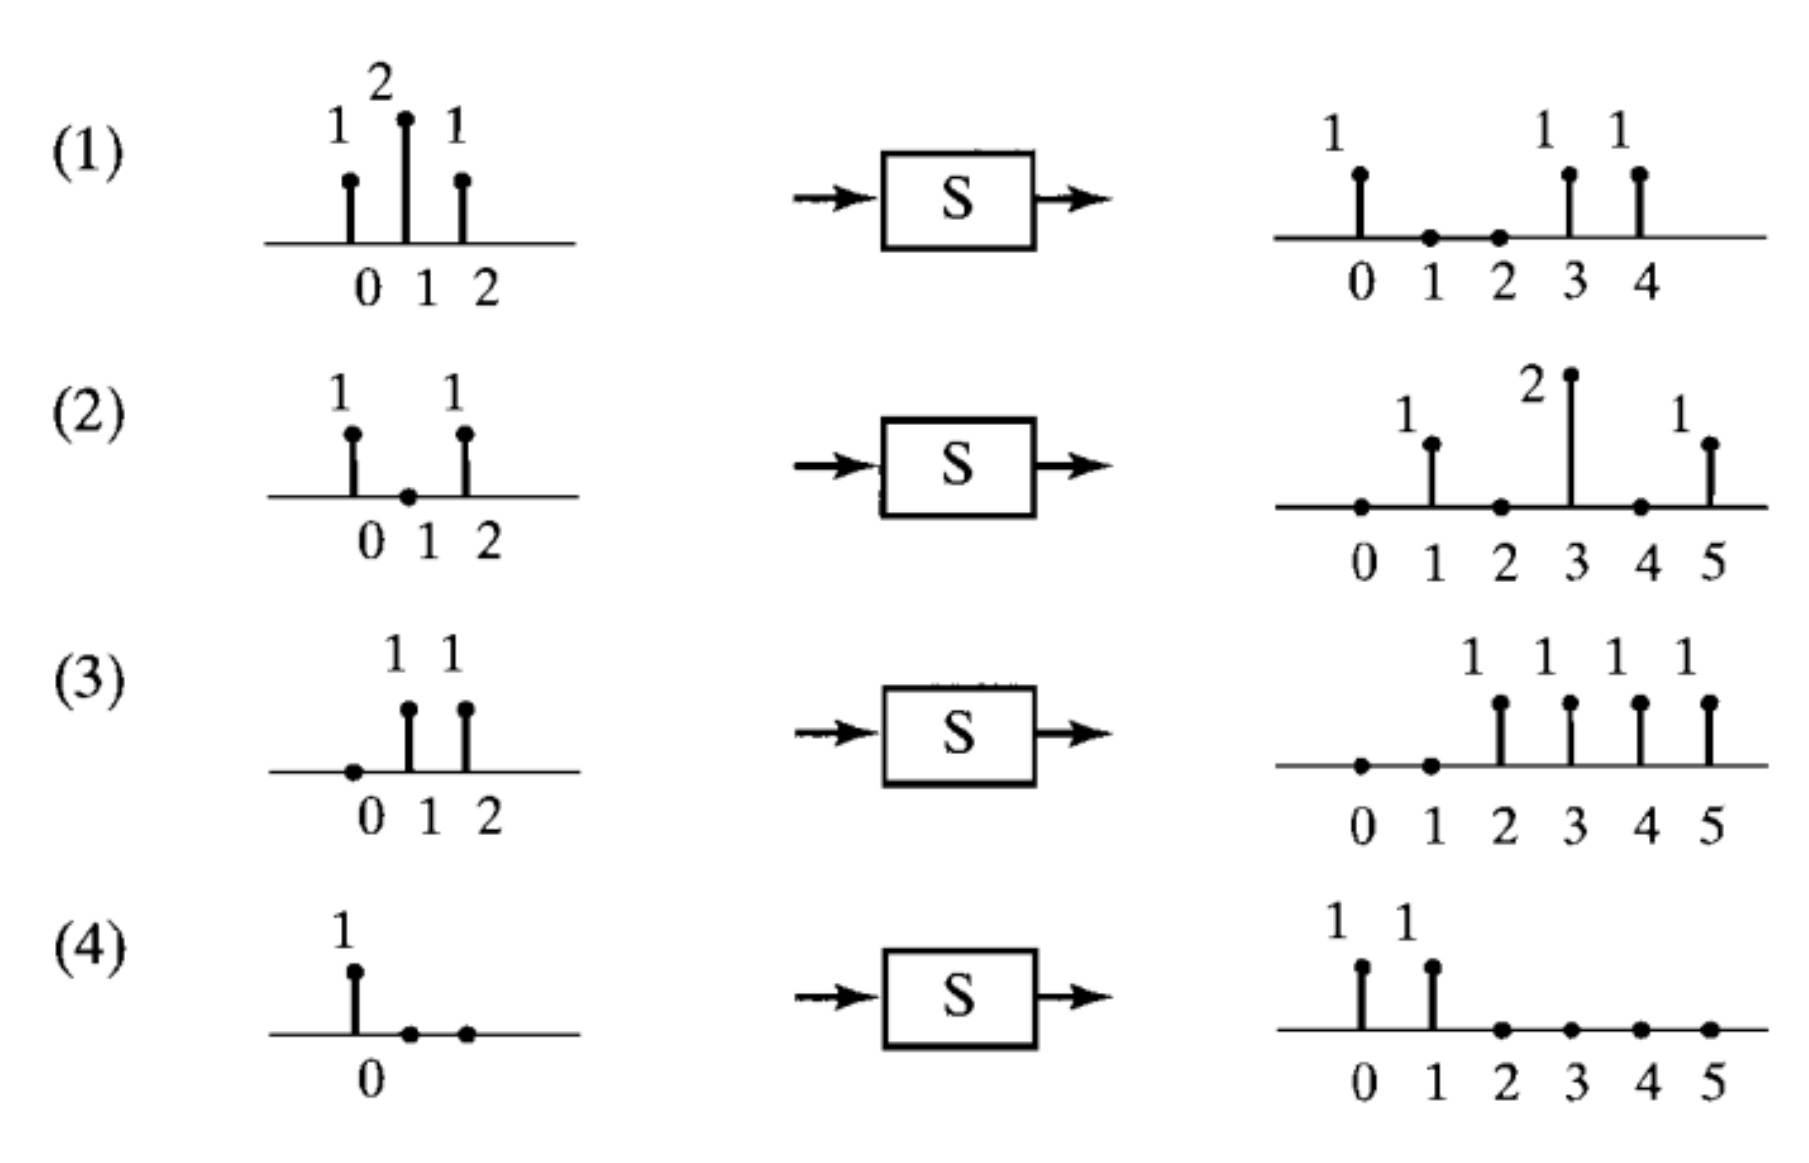
\includegraphics[scale=0.12]{Fig/q5.png}
\end{figure}
\subproblem \(S\) pode ser invariante no tempo? Explique.
\subproblem \(S\) pode ser linear? Explique.
\subproblem Se os pares de entrada-saída \((2)\) e \((3)\) fossem de um sistema LTI \(S_2\), qual seria a sua resposta impulsiva?
\subproblem Se os pares de entrada-saída \((1)\) for de um sistema LTI \(S_3\), qual seria a sua saída se o sinal de entrada fosse
\begin{figure}[H]
    \centering
    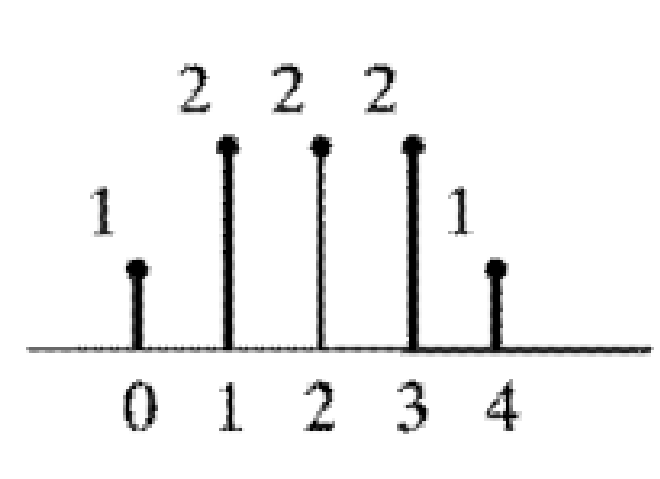
\includegraphics[scale=0.2]{Fig/q5_d.png}
\end{figure}

\problem Considere um sistema LTI de tempo discreto cuja resposta em frequência é dada por

\begin{equation}
H\left( e^{j\omega} \right) = \frac{\left( 1 - j e^{-j\omega} \right) \left( 1 + j e^{-j\omega} \right)}{1 - 0,8 e^{-j\omega}}
\end{equation}

Realize a expansão por frações parciais e obtenha \(h [n]\).

\problem Encontre a equação de diferenças para a resposta em frequência da questão anterior.

\problem Considere a resposta em frequência da questão 6, qual valor de \(\omega_0\) que o sinal de entrada, \(x [n] = 4 + 2 \cos{(\omega_0 n)}\), deve ter para que a saída do sistema seja uma constante? Qual é o valor dessa constante?

\problem Considere a equação

\begin{equation}
    x[n] = w[n] \cos{(\omega_0 n)},
\end{equation}
Em que \(w [n] = 1\) para \(|n| \leq L\).

\subproblem Calcule \(W\left( e^{j\omega} \right)\),  isto é, a DTFT de \(w [n]\).
\subproblem Calcule \(X\left( e^{j\omega} \right)\) em termos que \(W\left( e^{j\omega} \right)\)
\subproblem Esboçe o gráfico de \(X\left( e^{j\omega} \right)\)
\subproblem Explique a relação de \(L\) com a protuberância dos picos de \(X\left( e^{j\omega} \right)\)

\problem Considere um sistema que satisfaça a seguinte equações de diferenças
\begin{equation}
    x[n] = x[n] + 2x\left[ n-1 \right] + x\left[ n-1 \right]
\end{equation}

\subproblem Determine \(H\left( e^{j\omega} \right)\)
\subproblem Calcule \(h[n]\)
\subproblem O sistema é estável? Dica: Utilize as propriedades de estabilidade para justificar a sua resposta.
\subproblem Esboçe o gráfico de fase e magnitude de \(H\left( e^{j\omega} \right)\)

\end{document}
